%!TEX root = Main.tex
% System testing: words
\chapter{System Testing and Analysis} % (fold)
\label{cha:system_testing}

% Screenshots of data being sent and received (Logic)
% Timing analysis / diagrams

The testing methods and results are documented in this chapter.  The two primary blocks, described in the last chapter, were tested independently and then together, and will be presented here in the same manner.  A wide range of tools and techniques have been used to perform the testing, and to identify and fix errors encountered.

% Testing & things to document:
% x Testing methodology
% x GDP (software & hardware)
% x UART
% x SRAM (pre-tests, etc)
% x MFCCs
% Time of calculations, hardware vs software
% Full System - bus pirate, etc
% Hardware testing?? Current draw etc? .... Nah

\section{FPGA Design and Test Methodology} % (fold)
\label{sec:fpga_design_and_test_methodology}
	There were several phases of development, and thus testing, of this part of the design.  Initially, the full system was written and simulated in ModelSim, which supports SystemVerilog assertion based verification.  Each of the components of the design was built and tested separately, and then incrementally joined together and simulated as a whole.  Finally, the modules were tested in hardware -- first individually, and then as a full system.

	A set of testbenches were developed for use within ModelSim, which tested each of the modules used by the system.  Most of the modules were fairly simple to simulate and verify, as the expected behaviour is generally constant and determinate.  For example, verifying the UART clock generator was a case of instantiating it, asserting the enable signal, and verifying the frequency of the output signals.  However, some modules and their testbenches deserve extra attention, as special methods were used to test them.  In several areas, the benefits of using SystemVerilog become clear, as assertions greatly simplified the validation and testing process.

	Figure~\ref{fig:full_cycle} shows a simulation of the system performing a full cycle, from receiving an observation to sending back scores.
	\begin{figure}[tb]
		\begin{center}
			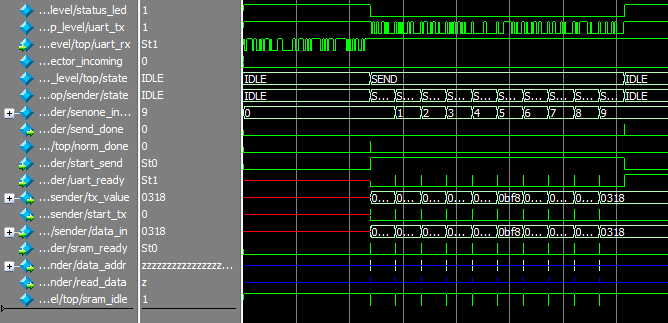
\includegraphics[width=\textwidth]{testbenches/full_cycle}
		\end{center}
		\caption{Simulation waveforms showing a full cycle of the top level state machine}
		\label{fig:full_cycle}
	\end{figure}
% section fpga_design_and_test_methodology (end)


\section{Gaussian Distance Calculation Block} % (fold)
\label{sec:gaussian_distance_calculation_testing}
	The Gaussian Distance Pipe was initially tested by creating a testbench which provided the sequence of inputs that the GDP required, and then asserted that the correct score was provided.  Figure~\ref{fig:test_gdp} shows the correct operation of this module, with a set of test data being used as inputs to the module.  The expected results were determined using the software GDP and the binary conversion software described in Section~\ref{sec:support_software}, thus confirming the validity of the results produced.

	\begin{figure}[tb]
		\begin{center}
			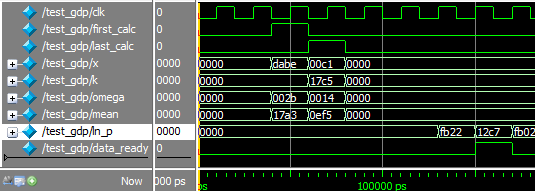
\includegraphics[width=\figwidth]{testbenches/gdp_wave}
		\end{center}
		\caption{GDP testbench waveform}
		\label{fig:test_gdp}
	\end{figure}
	
	The Gaussian Distance pipe controller testbench gives a new observation to the controller, and then watches as senone scores are produced by the module.  SystemVerilog assertions are used to check whether correct scores are arriving at the time they should.  However, in order to test a large number of different inputs (which would result in different score outputs), a set of software utilities were written to automatically generate the testbench code.  This software made use of the HMM definition parser and a software version of the GDP that had already been created.  This allowed a very large number of senones to be tested in a matter of minutes, and determine how well the GDP pipe was working.  Figure~\ref{fig:test_gdp_ctrl} shows the GDP Controller being tested.

	\begin{figure}[tb]
		\begin{center}
			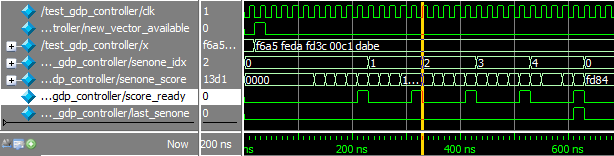
\includegraphics[width=\textwidth]{testbenches/gdp_ctrl_wave}
		\end{center}
		\caption{GDP Controller testbench waveform and error messages}
		\label{fig:test_gdp_ctrl}
	\end{figure}

	Being able to easily test many senones was important because the use of fixed-point arithmetic inevitably causes numerical errors that vary with the operations and numbers being used.  The GDP may produce the correct result for one set of inputs, but another set of inputs may produce an erroneous result that was caused by the fixed-point number not having high enough precision.  In fact, in most cases, the least significant bits of the result were wrong.  Because of this, it was important to determine the distribution of the error magnitudes, in order to decide whether the number format needed changing.  Automatic testbench generation made this far easier, as testbenches could be created which automatically displayed the senone scores that were wrong, and by how much.  The final system tolerated errors in the last 6 bits of the result, as this corresponds to less than 0.5\% of the total value.
	% TODO: talk about the error distribution??? I speak lots about how I found it (^) but don't actually say what the results were...


	From Figure~\ref{fig:test_gdp_ctrl}, it is also possible to observe the (ideal) time the GDP takes to calculate a score.  In this case (when \texttt{n\_components=5}), each senone takes 5 clock cycles (100ns with a 50MHz clock), after an initial pipeline loading delay.

	\subsection{Synthesis and Hardware Testing} % (fold)
	\label{sub:gdp_synthesis_and_hardware_testing}
		Unfortunately, due to the small size of the FPGA used, the initial synthesised design did not fit on it.  The full Voxforge model had over 7000 senones, and each observation had 25 parameters of 2 bytes each -- over 700kB of storage would be required for the full model.  As this far exceeds the resources available, the model size was reduced for the project.  The number of statistical parameters was reduced to 6, and only 12 senones were scored at once, bringing the FPGA slice usage to about 90\%.  % Confirmed.  Although at this %, may be clock skew!

		A variety of tools were used to repeatedly test the functionality of this hardware.  A Bus Pirate\footnote{Multi-purpose debugging tool that supports many different protocols.  See \href{http://dangerousprototypes.com/docs/Bus_Pirate}{http://dangerousprototypes.com/docs/Bus\_Pirate}} was used to communicate with the FPGA, which allows hexadecimal values to be easily sent and received over UART.  In order to debug the SystemVerilog, a large number of signals were routed to output pins, which were then monitored with a Saleae Logic analyser.
	% subsection gdp_synthesis_and_hardware_testing (end)
% section gaussian_distance_calculation_testing (end)


\section{UART Communications} % (fold)
\label{sec:uart_communications_testing}
	Simulating and testing the UART module was done by creating two instances of the module, and cross-connecting their RX and TX pins.  This allowed both transmit and receive to be tested, and confirmed correct operation.  An example of this testbench running is shown in Figure~\ref{fig:test_uart}.

	\begin{figure}[tb]
		\begin{center}
			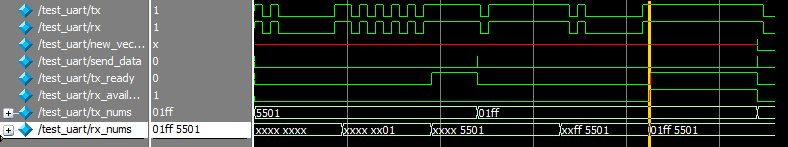
\includegraphics[width=\textwidth]{testbenches/uart_wave}
		\end{center}
		\caption{UART testbench waveform}
		\label{fig:test_uart}
	\end{figure}

	After simulation, the UART module was finally verified by programming the FPGA with the UART module, and a simple controller which echoed back whatever it received.  An FTDI USB to serial cable connected the FPGA to a computer, so that the setup could be confirmed to work with a real UART connection.  In addition, a Saleae Logic analyser was used to examine and ensure the absence of glitches in the UART signals generated by the FPGA.
% section uart_communications_testing (end)


\section{SRAM Access} % (fold)
\label{sec:sram_access_testing}
	A custom SystemVerilog module was designed in order to test writing and reading values to the SRAM chip, as it was a completely untested part of the board.  The module performed fairly basic operations, such as looping through a set of values, writing them to SRAM, and then reading them out again.  Debug information was displayed on the output pins, allowing the process to be monitored.  This confirmed that the chip worked as expected, and would be usable for the project.
% section sram_access_testing (end)


\section{Pre-Processing} % (fold)
\label{sec:pre_processing_testing}
	There were several different stages to the pre-processing, and these were tested individually.  First and foremost, the FFT code was tested by using input data containing known sinusoids.  The library used, FFTW, is well established and proven to work, and so the primary purpose here was to test the speed of the FFT.  It ran almost instantaneously (execution took 0.000000s, according to the Kernel time.h library), giving the correct results.

	The other major operation that required extensive testing was the MFCC calculation.  The other operations, pre-emphasis, windowing and liftering, are fairly straightforward mathematical operations that are easy to verify.  One of the desired properties of the system is that it would produce MFCCs that matched those produced by the HTK. Unfortunately, this was not quite achieved.  In most tests, the energy coefficient matched, but the others were relatively different.  This implies either that there is a limitation or problem with the MFCC library used, or that the HTK performs extra (or different) pre-processing.

	In addition, the library is very inefficient, causing the MFCCs to be produced relatively slowly.
% section pre_processing_testing (end)

\section{Software Based GDP Speed} % (fold)
\label{sec:software_based_gdp_speed_testing}
	The Gaussian Distance calculations were implemented in a C program in order to compare its performance with that of the FPGA.  It was found that the processor takes, on average, about 10$\mu s$ to calculate a single senone score -- about 100 times slower than the FPGA.  However, this version used double floating point precision, and thus is far more accurate than the FPGA.  Reducing the accuracy and using fixed-point values would definitely increase its speed.  % TODO!! Do this? It wouldn't be hard...
% section software_based_gdp_speed_testing (end)


% \section{Full system} % (fold)  % TODO
% \label{sec:full_system_testing}
% 	Once all the separate modules were tested and verified, the final task was to identify and eliminate the inevitable errors that occur once a design is integrated.

% % section full_system_testing (end)

% %!TEX root = Main.tex
% Project analysis: words
\chapter{Project Evaluation and Reflection} % (fold)
\label{cha:project_analysis}

This chapter presents an analysis of the final solution, evaluating its primary strengths and weaknesses, and the progress as a whole.

\section{Analysis of Solution} % (fold)
\label{sec:analysis_of_solution}

	\subsection{The FPGA} % (fold)
	\label{sub:analysis_the_fpga}
		The FPGA used was very small, and the full required design could not fit on it.  In particular, the size of the model had to be reduced, so that each Gaussian mean and variance had fewer than 25 components, and not all 7000 senones were processed.  However, what has been implemented is adequate to prove the concept, and demonstrate the advantages gained from using an FPGA.  In addition, it was known from the start that the full model would never fit, and so although this is a practical limitation, it does not make the project less worthwhile.

		Various benchmarks have been presented in the form of timing data.  It was shown that the FPGA was capable of calculating senone scores far faster than the traditional processor, albeit with an acceptable loss of accuracy.  This is similar to results achieved by Melnikoff \cite{melnikoff2003speech} and Speech Silicon \cite{schuster2006speech}, and supports the principle that custom-made hardware is faster than general purpose processors.  For real-time speech recognition, getting the senone scores as fast as possible is very important, as it allows more time for decoding tasks.  Thus, using an FPGA may be beneficial, especially in embedded systems.  It is possible to extrapolate, from the data gathered, the system speed when a larger model is implemented.  If the full model (7000 senones, 25 components) was used, the scores would be computed in about 3.5ms, leaving 6.5ms (of a 10ms window) for pre-processing and decoding (this excludes communications time).  If the embedded process was used to calculate the scores, it would take % TODO!!!! Recompile GDP-in-C with N_COMPS=25

		A big disadvantage of using an FPGA, in such a system, is the need to communicate to it.  The communication is an added step that adds time to the senone scoring process, and, if it is not fast enough, may render the use of an FPGA not worthwhile.  The implemented communication method (UART) is extremely slow and is the weakest point of the system, as is obvious in Figure~\ref{fig:full_cycle} which shows a complete cycle of the top level state machine.  Although it is not visible, the state machine goes through PROC and GDP, but these stages are far faster than the UART communication.  UART was used primarily for the ease of implementation, and because at this stage real-time operations are not required.  However, for this system to be realistically useful, a better communication method needs to be developed -- either a far faster serial bus or some form of hybrid serial-parallel connection.

		\begin{figure}[tb]
			\begin{center}
				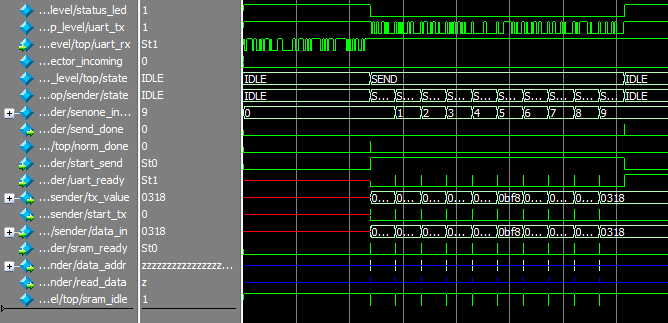
\includegraphics[width=\textwidth]{testbenches/full_cycle}
			\end{center}
			\caption{Simulation waveforms showing a full cycle of the top level state machine}
			\label{fig:full_cycle}
		\end{figure}

		% Additionally, the number format used caused the calculation accuracy to be reduced
	% subsection the_fpga (end)

	% Evaluate the speed - how long did each cycle take.  How much time was added by adding another component? or another senone? Extrapolate?

	\subsection{The Processor} % (fold)
	\label{sub:analysis_the_processor}
		The biggest problem, or limitation, with the current preprocessing system is the MFCC calculation step.  The external LibMFCC library is not optimised for the project's requirements at all, but it was convenient, and serves its purpose.  The HTK has a far faster implementation of this step, and could have been ported to the project code, had more time been available.

		However, what has been implemented is a good demonstration of the capabilities of this processor, and how it is capable of working with the FPGA.
	% subsection the_processor (end)


\section{Deviations from Original Goals} % (fold)
\label{sec:deviations_from_original_goals}
	Originally, while planning the project, the goal had been to implement a complete speech recognition system, from pre-processing to Viterbi decoding (see Appendix~\ref{apdx:brief}).  However, as more was learnt about the systems involved, it became clear that it was far too large a subject to attack in a single project.  Thus, the biggest change from initial plans was to narrow the project's focus down to a particular area of speech recognition.  However, with respect to the focussed goal, the results achieved are very satisfactoy.

	Development began by following the Gantt chart in Appendix~\ref{apdx:gantt_chart1}, which was also presented in the project Interim Report.  However, when building a software decoder proved to be far more time consuming than expected, the decision was made to change the focus, as mentioned above.  
	The remaining progress followed the Gantt chart in Appendix~\ref{apdx:gantt_chart2}\footnote{Both Gantt charts were created and modified using Gantter (http://app.gantter.com)}.  The majority of the design and implementation was completed in a timely manner, thus showing that the revised goals were more realistic.
% section deviations_from_original_goals (end)


% section analysis_of_solution (end)

% chapter project_analysis (end)

% chapter system_testing (end)